\documentclass[a4paper,12pt]{article}
\usepackage{listings}  %cpp code
\usepackage[T1,T2A]{fontenc}
\usepackage[utf8]{inputenc}
%\renewcommand{\rmdefault}{ftm}-TimesNewRoman
\usepackage[14pt]{extsizes}
\usepackage[ukrainian]{babel}
\usepackage{amsmath}
\usepackage{tikz}
\usepackage{pgfplots}
\usepackage{gnuplottex}
\usepackage{graphicx}
\usepackage{gensymb}
\usepackage{graphicx}
\usepackage{subcaption}
\graphicspath{{pictures/}}
\DeclareGraphicsExtensions{.pdf,.png,.jpg,.gif}
\pgfplotsset{compat = 1.3}
\sloppy %-rastiazhenie abzaca
\relpenalty=10000
\pagestyle{plain}
\begin{document}
\title{\HugeЗвіт до лабораторної роботи №2\linebreak }
\author{\LargeВиконали: Дирів Олександр та Рябоконь Максим}
\date{}
\maketitle
\newpage
{\Large\tableofcontents}
\newpage
\section{Інтегруючий чотириполюсник}
\quad Схема RC чотириполюсника (Рис. 1) 
\par\quad\begin{figure}[!h]
  \centering
 \begin{subfigure}[b]{0.6\linewidth}
    \includegraphics[width=\linewidth]{p1.png}
  \end{subfigure}
  \caption{}
\end{figure}
\par\quad Розрахуємо його амплітудно-частотну та фазо-частотну характеристику. З формули (Рис. 2) визначається амплітудно-частотна та фазово частотна характеристики.  
\par\quad\begin{figure}[!h]
  \centering
 \begin{subfigure}[b]{0.6\linewidth}
    \includegraphics[width=\linewidth]{f2.png}
  \end{subfigure}
  \caption{}
\end{figure}
\clearpage
\quad Для дослідження перехідних характеристик необхідно подати на вхід прямокутний сигнал (меандр). Звідси можна знайти час наростання імпульсу приблизно 50ms. За допомогою перетворення Лапласа можна показати, що залежність напруги на виході від часу виражається експонентою для обох чотириполюсників. 
\par\quad\begin{figure}[!h]
  \centering
 \begin{subfigure}[b]{1\linewidth}
    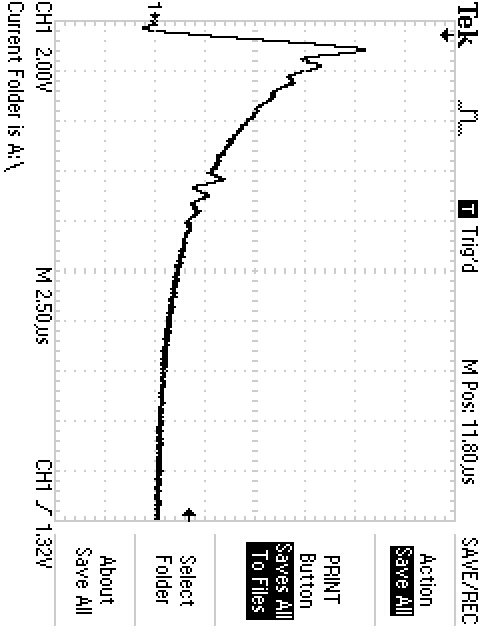
\includegraphics[width=\linewidth]{F0001TEK.JPG}
  \end{subfigure}
  \caption{}
\end{figure}
\par\quad\begin{figure}[!h]
  \centering
 \begin{subfigure}[b]{1\linewidth}
    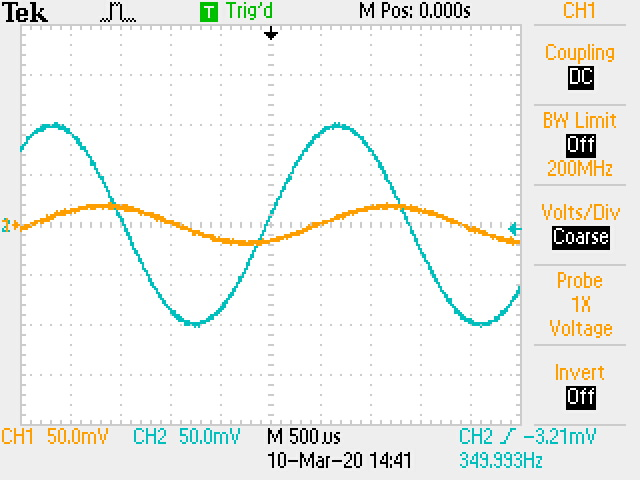
\includegraphics[width=\linewidth]{F0003TEK.JPG}
  \end{subfigure}
  \caption{}
\end{figure}
\clearpage
\section{Диференціюючий чотириполюсник}
\quad Схема CR чотириполюсника (Рис. 5) 
\par\quad\begin{figure}[!h]
  \centering
 \begin{subfigure}[b]{0.6\linewidth}
    \includegraphics[width=\linewidth]{p2.png}
  \end{subfigure}
  \caption{}
\end{figure}
\par\quad Розрахуємо його амплітудно-частотну та фазо-частотну характеристику. З формули (Рис. 6) визначається амплітудно-частотна та фазово частотна характеристики.  
\par\quad\begin{figure}[!h]
  \centering
 \begin{subfigure}[b]{0.6\linewidth}
    \includegraphics[width=\linewidth]{f1.png}
  \end{subfigure}
  \caption{}
\end{figure}
\clearpage
\par\quad Для дослідження перехідних характеристик необхідно подати на вхід прямокутний сигнал (меандр). Звідси можна знайти час наростання імпульсу приблизно 50ms.  
\par\quad\begin{figure}[!h]
  \centering
 \begin{subfigure}[b]{1\linewidth}
    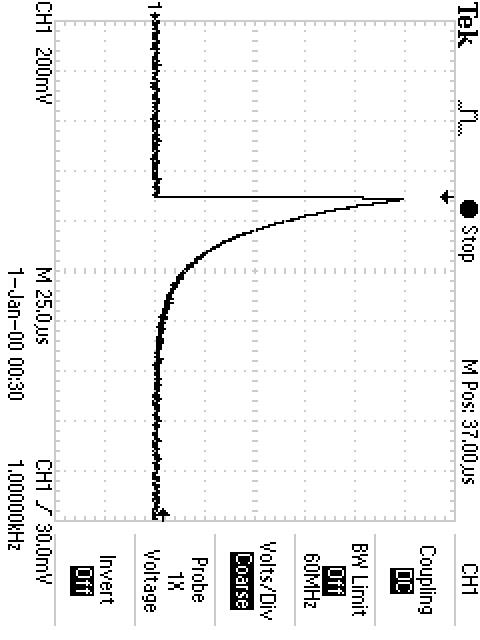
\includegraphics[width=\linewidth]{F0000TEK.JPG}
  \end{subfigure}
  \caption{}
\end{figure}
\par\quad\begin{figure}[!h]
  \centering
 \begin{subfigure}[b]{1\linewidth}
    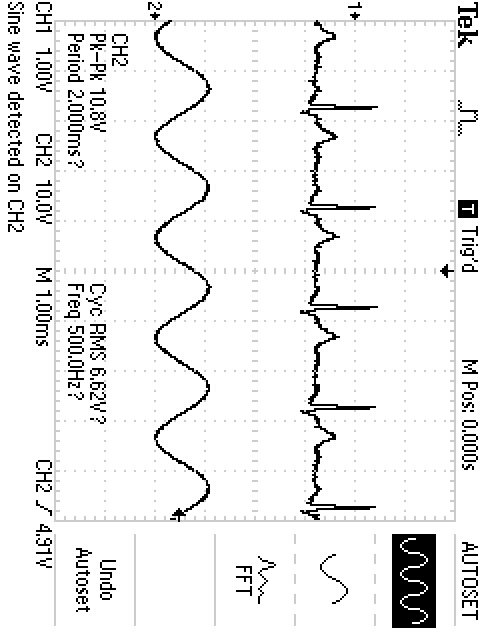
\includegraphics[width=\linewidth]{F0005TEK.JPG}
  \end{subfigure}
  \caption{}
\end{figure}
\clearpage
\section{Висновки}
\par\quadУ результаті даної лабораторної роботи були досліджені перехідні характеристики чотириполюсників та побудовані їх теоретичні розрахунки. Загалом виникали деякі відхилення від теорії за рахунок паразитних імпедансів. На жаль частотні характеристики ми не встигли дослідити.
\end{document}